\chapter{Cobordism groups}\label{Cob Groups}
We now define the most fundamental object in cobordism theory: the cobordism group.
 It is an algebraic structure characterizig if two manifolds are cobordant and how this relates to the
  disjoint 
 union of manifolds. From this one can establish cobordism invariants, i.e. homomorphisms 
 from a certain cobordism group to another abelian group. To do this, we will exploit
 the classifications of 1- and 2-manifolds up to diffeomorphism we proved in the previous chapters.
  To be diffeomorphic is a much 
 stricter and finer relation then being cobordant, that is why it is much harder to classify manifolds
 up to diffeomorphism, but it also will make our life much easier when establishing cobordism invariants.
\begin{defn}
    \label{Defn n-th cob group}
    The set underlying the $n$-th cobordism group is
    $$\Omega_n = \frac{\{\text{closed $n$ manifolds}\}}{\{\text{$n+1$ cobordisms}\}}$$
    $(\Omega_n, \amalg)$ is an abelian group with operation given by the disjoint union $\amalg$.
    \begin{enumerate}
        \item the disjoint union is associative and commutative
        \item the identity element\footnote{We will
            sometimes write $0=[\emptyset]$ or more often $\emptyset=[\emptyset]$}
        is the cobordism class of the empty set\footnote{Reminder: $\emptyset$ is an $n$-manifold for every $n$.}
        $[\emptyset]$, i.e. the set of $n$-manifolds which are bordant with the empty set
        \item every element has an inverse:
        $[M]\amalg [M]=[\emptyset]$ since $M\amalg M=(\de(M\times[0,1]))$ and such a cylinder can be bent into a
        macaroni, which is bordant to the empty set:
        \[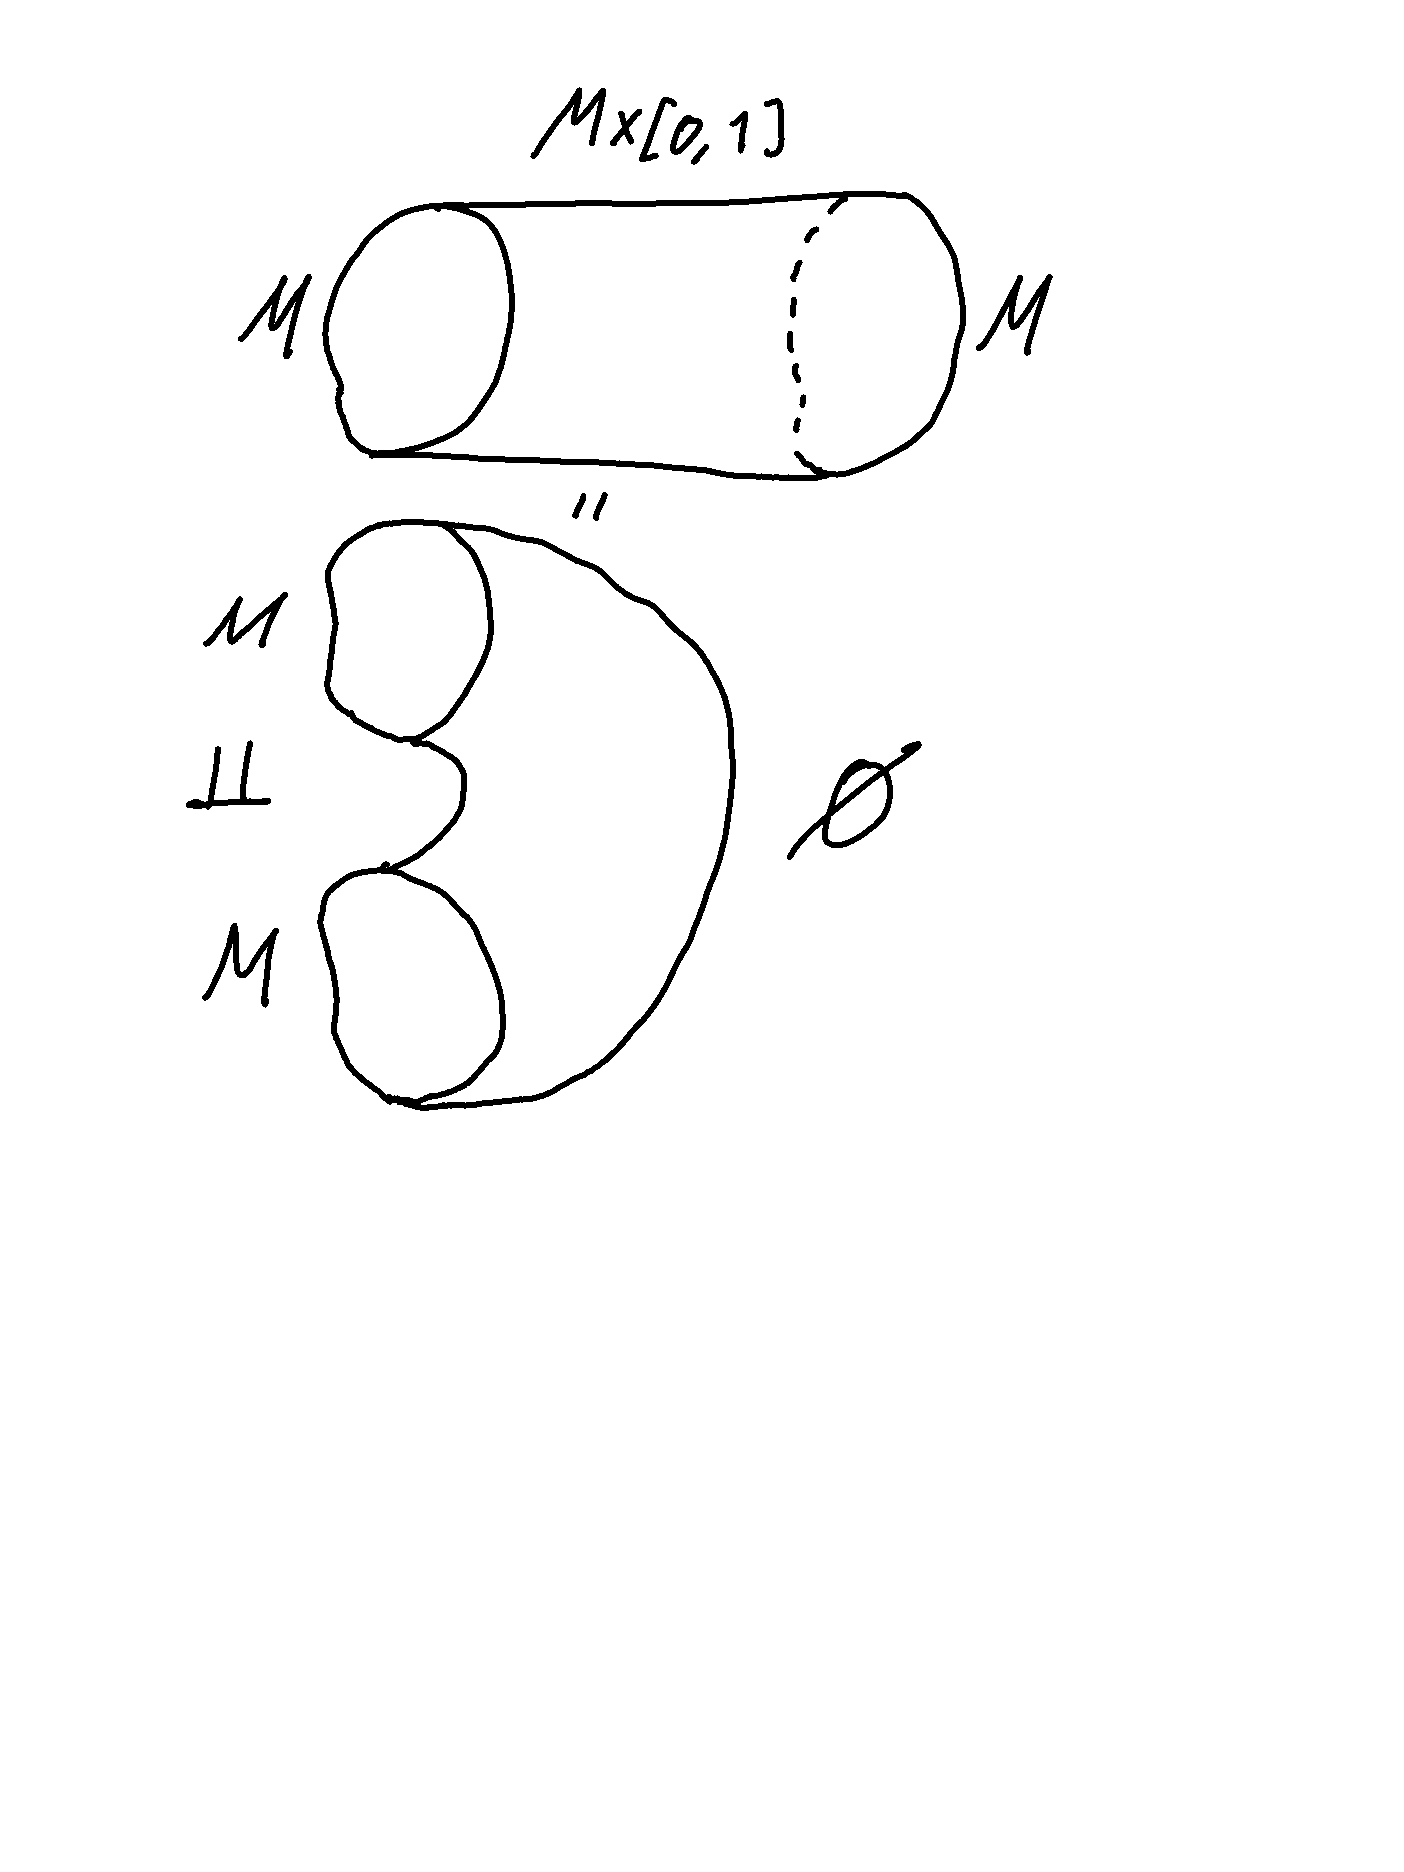
\includegraphics[width=6.5cm]{images/Lecture 2/MACARONI.png}\]
    \end{enumerate}
\end{defn}
\begin{rem}
    There is an insidious set-theoretic issue when we define the $n$-th cobordism group $\Omega_n$ (\ref{Defn n-th cob group}): is the collection of all closed $n$-manifolds a set? And what about the collection of all $(n+1)$-bordisms? It could be the case that it is something bigger than a usual set, thus not a set and problematic since we would not know how to treat them\footnote{We are assuming to be working in ZFC. There are other set theories in which one can define collections greater than sets, e.g. Von Neumann–Bernays–Gödel set theory.}. For example, we know that the collection of all sets is strictly greater than any set\footnote{Because of famous set-theoretic paradoxes like Cantor's paradox.} and thus not a set. Similarly, also the collection of topological spaces is not a set because we can regard any set as a topological space via the discrete topology\footnote{The topology where the set of open sets is the powerset of the set in question, or in other words where any subset is open.}. One could wonder if the collection of all manifolds of a certain dimension $n$ is likewise not a set. This is fortunately for us not the case. The following theorem allows us to happily treat \{\text{closed $n$ manifolds}\} and \{\text{$n+1$ cobordisms}\} as sets by replacing abstract manifolds and cobordism by manifolds and cobordisms embedded in $\R^{\infty}$.
\end{rem}
\begin{thm}[Whitney Embedding theorem\footnote{This result is not important only in this case, but notably for the interest of this class it was used to construct an apt category of bordisms \ref{CobCat} in order to sketch a partial proof of the most important conjecture in the field of TFTs: the cobordism hypothesis; see for details on this \cite{lurie2009classification} and \cite{Calaque_2019}.}]
    Any $n$ manifold can be embedded in $\R^{\infty}(=\bigcup_{n\in\N}\R^n)$. The space of such embeddings is contractible.\footnote{Note that there are refinements of the latter result.}
\end{thm}

\begin{rem}
    Actually $(\Omega_n,\amalg)$ is a finitely generated abelian group, but this is a hard theorem. In particular, it is a finite product of cyclic groups of order $2$ (from 2.)
\end{rem}

\begin{defn}[Bordism invariant]
    A bordism invariant is a homomorphism of abelian groups $$(\Omega_n,\amalg,\emptyset) \to (A,\cdot,e)$$ 
    the abelian group $A$ can be $\Z$, $\R$ or $\C$ for instance.
\end{defn}
\begin{rem}
    Many important manifold invariants are also bordism invariants.
\end{rem}

\begin{ex}
    \hfill
    \begin{itemize}%TODO complete
        \item $\chi$ mod 2 (the Euler characteristic)
        \item signature
        \item characteristic classes such as Pontrjagin, Stiefel-Whitney or Chern classes 
    \end{itemize}
\end{ex}
%TODO add definition of characteristic class or maybe just some additional comment
\section{The 0-th Cobordism Group, \texorpdfstring{$\Omega_{0}$}{Omega 0}}
Consider
$$\Omega_0 = \{\text{finite disjoint unions of points}\} / \{\text{$1$-dimensional cobordisms}\}.$$
To compute this, consider the following classification of $1$ manifolds:

\begin{prop}\label{prop:classification_1d}
    Any $1$ dimensional compact manifold with boundary is diffeomorphic to a finite disjoint union of closed intervals $[0,1]$ and circles $S^1$.
\end{prop}
%TODO add proof, it should not be hard, and useful also for classification of 1TFT
\begin{ex}
    An example of a $1$-dimensional cobordism is $W=[0,1]$. Here are the 3 different way of seeing it as a bordism: from $Y_0 = \{0,1\}$ to $Y_1 = \emptyset$, from $Y_0 = \{0\}$ to $Y_1 = \{1\}$ and from $Y_0 = \emptyset$ to $Y_1 = \{0,1\}$.
    \begin{figure}[H]
        \centering
        \begin{tikzpicture}
            % Line segment
            \draw[line width=1pt] (0,0.5) arc (90:270:-0.5 and 0.5);
            
            % Filled dots at the ends
            \fill (0,0.5) circle (2pt);
            \fill (0,-0.5) circle (2pt);
            
            \draw[line width=1pt] (3.5,0) -- (4.5,0);
            
            % Filled dots at the ends
            \fill (3.5,0) circle (2pt);
            \fill (4.5,0) circle (2pt);
            
            \draw[line width=1pt] (8,0.5) arc (90:270:0.5 and 0.5);
            
            % Filled dots at the ends
            \fill (8,0.5) circle (2pt);
            \fill (8,-0.5) circle (2pt);
        \end{tikzpicture}
        %\caption{}
    \end{figure}
\end{ex}

\begin{ex} Here is a list of various finite disjoint unions of points with different cardinalities. Can you see a pattern emerging?
    \begin{figure}[H]
        \captionsetup[subfigure]{labelformat=empty}
        \centering
        \begin{subfigure}[t]{.3\textwidth}
            \centering
            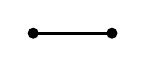
\begin{tikzpicture}
                \draw[line width=1pt] (0,0) -- (1,0);
                
                \fill (0,0) circle (2pt);
                \fill (1,0) circle (2pt);
            \end{tikzpicture}
            \caption{1 point}
        \end{subfigure}
        %
        \begin{subfigure}[t]{.3\textwidth}
            \centering
            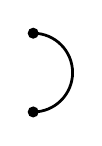
\begin{tikzpicture}
                \draw[line width=1pt] (0,0.5) arc (90:270:-0.5 and 0.5);
                
                \fill (0,0.5) circle (2pt);
                \fill (0,-0.5) circle (2pt);
            \end{tikzpicture}
            \caption{2 points}
        \end{subfigure}
        %
        \begin{subfigure}[t]{.3\textwidth}
            \centering
            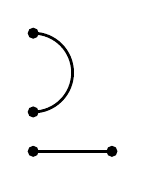
\begin{tikzpicture}
                \draw[line width=1pt] (0,0.5) arc (90:270:-0.5 and 0.5);
                
                \fill (0,0.5) circle (2pt);
                \fill (0,-0.5) circle (2pt);
                
                \draw[line width=1pt] (0,-1) -- (1,-1);
                
                \fill (0,-1) circle (2pt);
                \fill (1,-1) circle (2pt);
            \end{tikzpicture}
            \caption{3 points}
        \end{subfigure}
        
        \bigskip
        
        \begin{subfigure}[t]{.3\textwidth}
            \centering
            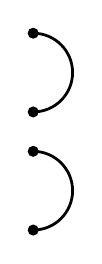
\begin{tikzpicture}
                % Line segment
                \draw[line width=1pt] (0,0.5) arc (90:270:-0.5 and 0.5);
                
                % Filled dots at the ends
                \fill (0,0.5) circle (2pt);
                \fill (0,-0.5) circle (2pt);
                
                % Line segment
                \draw[line width=1pt] (0,-1) arc (90:270:-0.5 and 0.5);
                
                % Filled dots at the ends
                \fill (0,-1) circle (2pt);
                \fill (0,-2) circle (2pt);
            \end{tikzpicture}
            \caption{4 points}
        \end{subfigure}
        %
        \begin{subfigure}[t]{.3\textwidth}
            \centering
            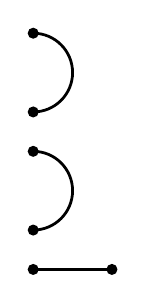
\begin{tikzpicture}
                % Line segment
                \draw[line width=1pt] (0,0.5) arc (90:270:-0.5 and 0.5);
                
                % Filled dots at the ends
                \fill (0,0.5) circle (2pt);
                \fill (0,-0.5) circle (2pt);
                
                % Line segment
                \draw[line width=1pt] (0,-1) arc (90:270:-0.5 and 0.5);
                
                % Filled dots at the ends
                \fill (0,-1) circle (2pt);
                \fill (0,-2) circle (2pt);
                
                % Line segment
                \draw[line width=1pt] (0,-2.5) -- (1,-2.5);
                
                % Filled dots at the ends
                \fill (0,-2.5) circle (2pt);
                \fill (1,-2.5) circle (2pt);
            \end{tikzpicture}
            \caption{5 points}
        \end{subfigure}
        %
        \begin{subfigure}[t]{.3\textwidth}
            \centering
            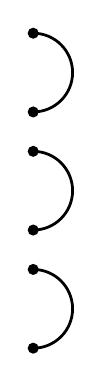
\begin{tikzpicture}
                % Line segment
                \draw[line width=1pt] (0,0.5) arc (90:270:-0.5 and 0.5);
                
                % Filled dots at the ends
                \fill (0,0.5) circle (2pt);
                \fill (0,-0.5) circle (2pt);
                
                % Line segment
                \draw[line width=1pt] (0,-1) arc (90:270:-0.5 and 0.5);
                
                % Filled dots at the ends
                \fill (0,-1) circle (2pt);
                \fill (0,-2) circle (2pt);
                
                % Line segment
                \draw[line width=1pt] (0,-2.5) arc (90:270:-0.5 and 0.5);
                
                % Filled dots at the ends
                \fill (0,-2.5) circle (2pt);
                \fill (0,-3.5) circle (2pt);
            \end{tikzpicture}
            \caption{6 points}
        \end{subfigure}
    \end{figure}
\end{ex}

\noindent Keeping this pattern in mind, consider collection of $k$ points, with $k$ finite (i.e. the only closed 0 manifolds):

\begin{itemize}
    \item If $k$ is even, we can find a bordism to $\emptyset$
    \item If $k$ is odd, we can find a bordism to $\{*\}$
\end{itemize}

\noindent We then have 
\begin{equation*}
    2k \text{ points} \sim \emptyset, \quad\quad 2k+1 \text{ points} \sim \text{1 point}
\end{equation*}
Therefore, the 0-th cobordism group is given by
\begin{equation}
    \Omega_0 = \{ \emptyset, \{*\}\} \cong \Z_2.
\end{equation}
A possible variation is: add a ``decoration'', called \textit{orientation} (will be made more precise later), so we now have:
$$\Omega_0^{\textit{or}} = \big\{\text{finite sets of points $S$ with a map } S \to \{+,-\}\big\} /\{\text{oriented cobordism}\}$$

An oriented cobordism in $1$ dimension is given by $[0,1]$ or $S^1$ which comes with an orientation. Here are some
examples

\[ 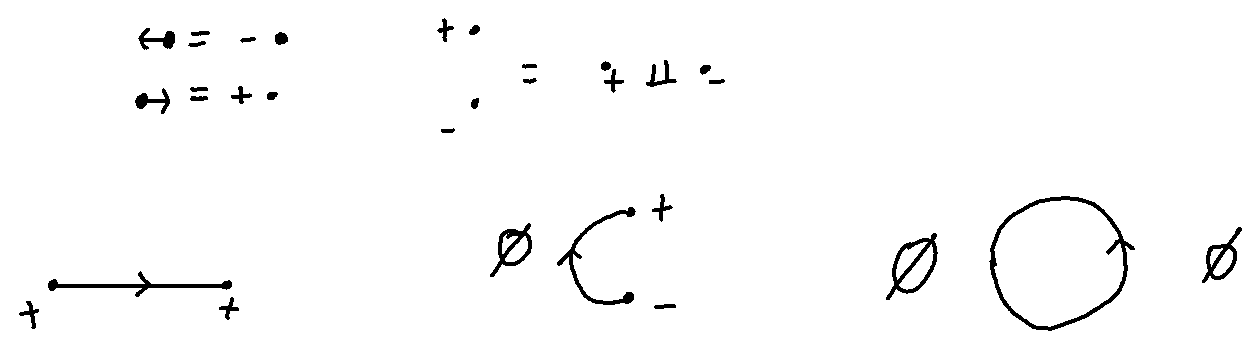
\includegraphics[width=9cm]{images/Lecture 11/1dBORDISM.png}\]

\begin{exercise}
    What is $\Omega_0^{or}$? Try to think about it! 
\end{exercise}

\subsection{The 1st cobordism group, \texorpdfstring{$\Omega_{1}$}{Omega 1}}
Now we have
$$\Omega_1= \{\text{closed $1$-dimensional manifolds}\} / \{\text{$2$-dimensional cobordisms}\}.$$
In studying this group, the following result, which is a restriction of \ref{prop:classification_1d}:
\begin{thm}
    
    Any closed $1$-dimensional manifold is a finite disjoint union of circles
\end{thm}
\noindent However, a circle is the boundary of a 2-disk, which gives a cobordism from $S^1$ to $\emptyset$, we then have $S^1 \sim \emptyset$. Hence, also finite disjoint unions of $S^1$ are cobordant to the empty set. Therefore, the $1$st cobordism group is trivial:
\begin{equation}
    \Omega_1 = 0
\end{equation}

\section{The 2nd cobordism group, \texorpdfstring{$\Omega_{2}$}{Omega 2}}
In order to find the $2$nd cobordism group, we first need a classification of $2$ manifolds. %(Introduced before) In order to state the result we need to introduce the concept of \textit{connected sum}
%\begin{defn}[Connected Sum]
%Given $n$ manifolds $M,N$, their connected sum $M\# N$ is given by
%%M\# N = M \setminus (D^n)^\circ \cup_{\de D^n \times [0,1]} N \setminus (D^n)^\circ
%\end{equation}
%\end{defn}
%DRAWING
\begin{prop}[Classification of $2$-dimensional manifolds]\label{Classification of 2 manifolds}
    Every connected closed $2$ manifold is diffeomorphic to
    \begin{enumerate}
        \item $S^2$, orientable
        \begin{figure}[!ht]
            \centering
            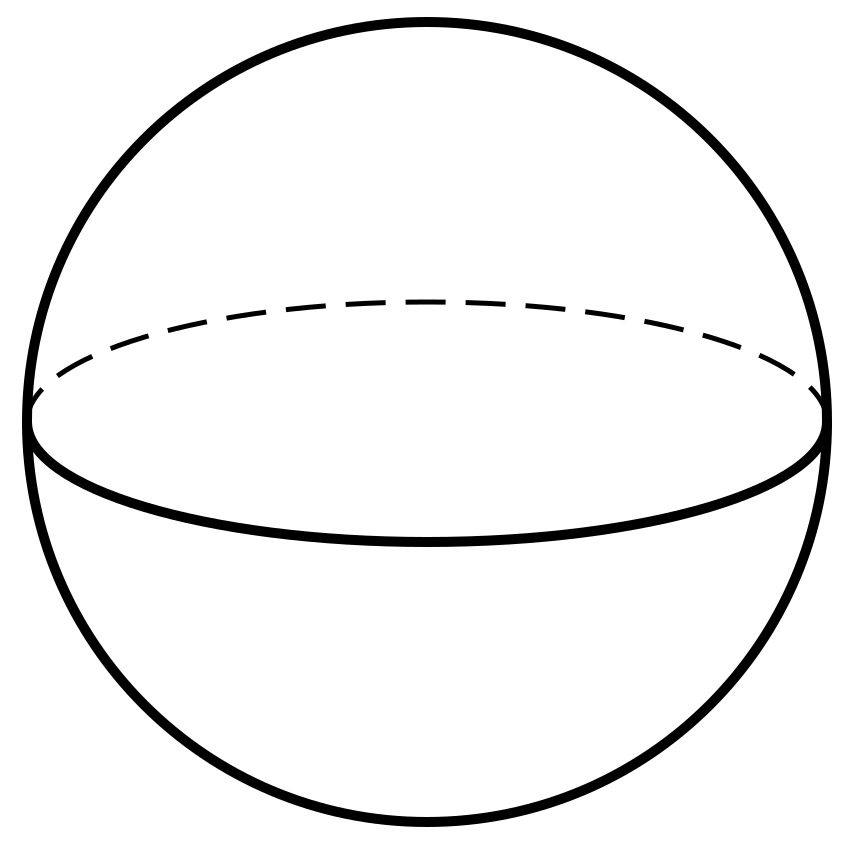
\includegraphics[width=3cm]{images/Lecture 3/sphere.png}
            \caption{2-sphere, $S^2$}
        \end{figure}
        \item $\Sigma_g = \underbrace{T \# \dots \# T}_{g-\text{times}}$ , orientable
        \begin{figure}[!ht]
            \centering
            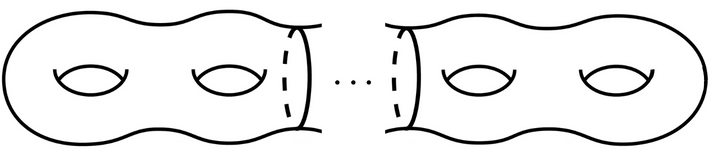
\includegraphics[width=10cm]{images/Lecture 3/surface_of_genus_g.png}
            \caption{Surface of genus g, $\Sigma_g$}
        \end{figure}
        \item $P_k = \underbrace{\R\P^2 \# \dots \# \R\P^2}_{k-\text{times}}$ , non-orientable
        \begin{figure}[!ht]
            \centering
            \begin{subfigure}[t]{.4\textwidth}
                \centering
                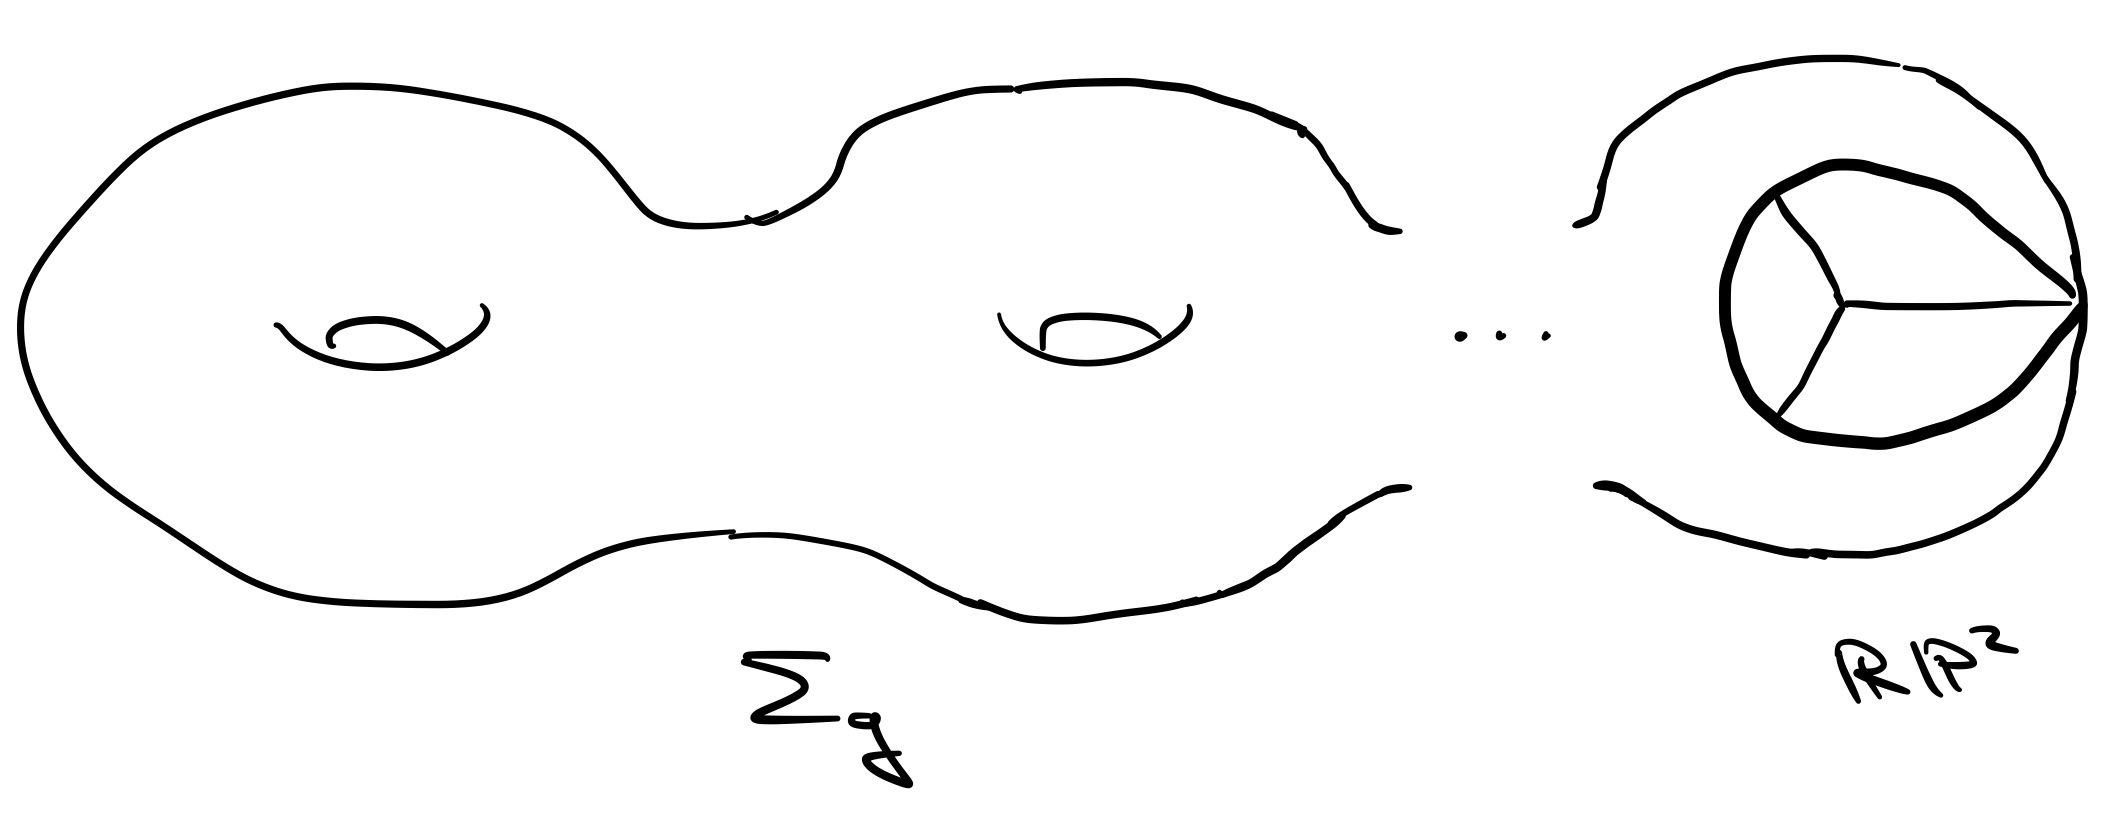
\includegraphics[width=6cm]{images/Lecture 3/sigma_g_rp2.png}
                \caption{$P_{2g+1} \cong \Sigma_g \# \R\P^2$}
            \end{subfigure}\hspace{10mm}
            \begin{subfigure}[t]{.4\textwidth}
                \centering
                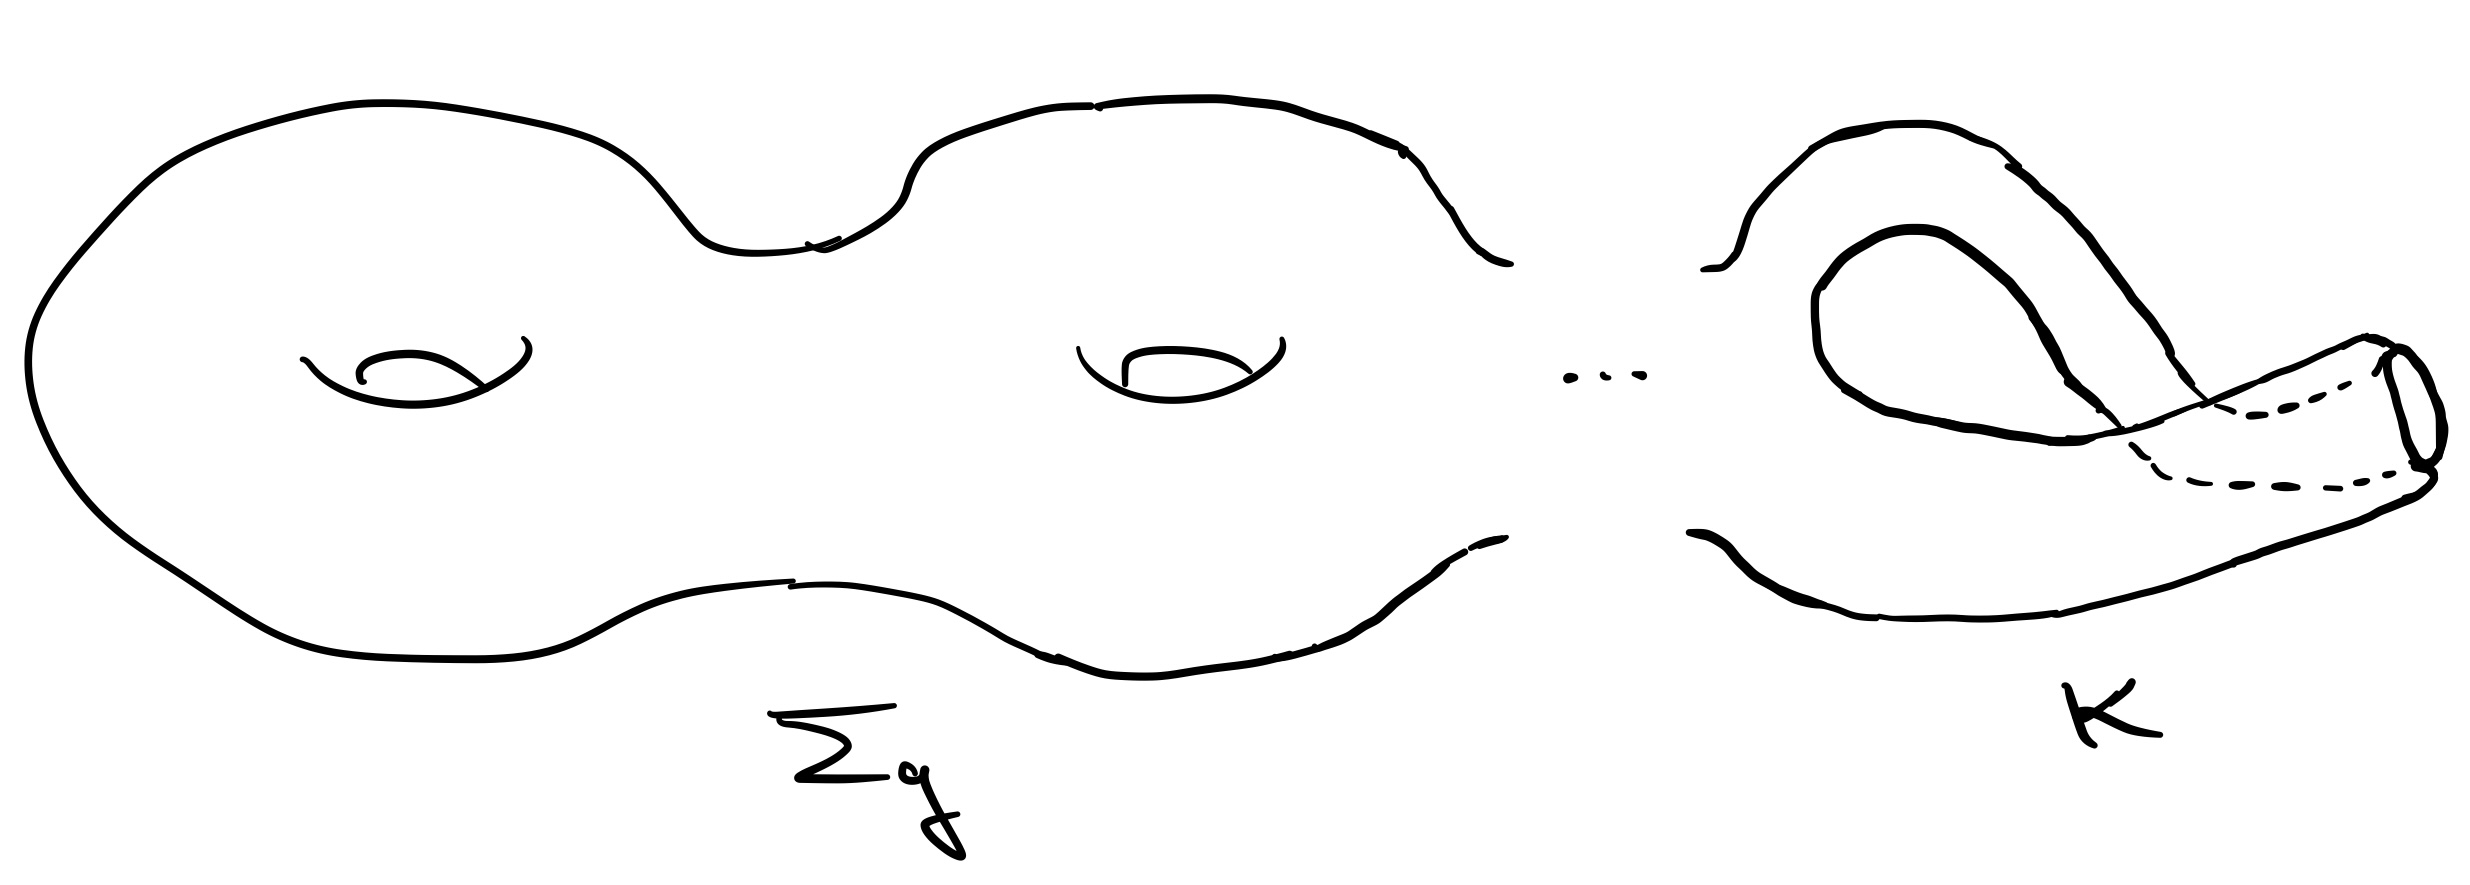
\includegraphics[width=6cm]{images/Lecture 3/sigma_g_klein_bottle.png}
                \caption{$P_{2g+2} \cong \Sigma_g \# K$}
            \end{subfigure}
        \end{figure}
    \end{enumerate}
\end{prop}

\noindent We can now use this knowledge to compute
$$
\Omega_2^{\text{or}} = \{\text{closed oriented $2$ manifolds} \} /\{\text{$3$-dimensional oriented cobordisms}\}
$$
by observing that $S^2$ and $\Sigma_g$ are both cobordant to $\emptyset$ since they can simply be ``filled'' to a $3$ dimensional manifold with boundary, we get
\begin{equation}
    \Omega_2^{or} = 0.
\end{equation} 
%DRAWING
\begin{exercise}
    What about the non-oriented part $\Omega_2$?
\end{exercise}

%Can this go with the cobordism part? /William YES, I agree that it makes much more sense and that is why I am restructuring some stuff /Andrea
\section{More on cobordism groups}
\label{sec:more_on_cobordism_groups}

We now go back to cobordism groups to give some important results.

We had found 
\begin{align}
    &\Omega_0 \cong \Z_2 \\
    &\Omega_1 \cong 0    \\
    &\Omega_2 \cong \Z_2
\end{align}
while for the oriented case we have
\begin{align}
    &\Omega_0^{or} \cong \Z \\
    &\Omega_1^{or} \cong 0  \\
    &\Omega_2^{or} \cong 0
\end{align}
\begin{defn}[Commutative \Z-Graded Ring\footnote{Note that there is a difference between commutative graded ring and graded commutative ring! A commutative graded ring is a commutative ring that is graded (our notion), a graded commutative ring is a different notion that depends on the degree of homogeneous elements.}]
A commutative \Z-graded ring is a ring $R$ if there is a family of subgroups $\{R_n\}n\in\Z$ such that 
\begin{itemize}
\item the underlying abelian group can be decomposed as $R=\bigoplus_{n \in \Z} R_n$
\item $R_n \cdot R_k \subset R_{n+k}$ for all $n,k\in\Z)$
\end{itemize}
A non-zero element $x\in R_n$ is called a homogeneous element of $R$ of degree $n$.
\end{defn}

\begin{prop}
    $(\Omega_\bullet = \bigoplus_{n\geq 0} \Omega_n, \amalg, \times)$ is a commutative \Z-graded ring.
\end{prop}
\begin{proof}
    Firstly we need to check that the product respects the degree: this is true because $M^m \times N^n = (M \times N)^{m+n}$, so $[M\times N] \in \Omega_{m+n}$.

    \noindent Then the products descends to equivalence classes: if $Y_0 \simeq Y_1$ are cobordant via cobordism $(X,p)$ ($p:\de X \to {0,1}$), $M$ any manifold, then $\de X \times M = \de X \times M \xrightarrow{p \circ pr_X} \{0,1\}$. Therefore $(X \times M, p \circ pr_X)$ is a cobordism from $Y_0 \times M$ to $Y_1 \times M$.
\end{proof}

\begin{thm}[Thom]
    There is an isomorphism of \Z-graded commutative rings
    \begin{equation}
        \Omega_\bullet \cong \Z_2[x_2, x_4, x_5, x_6, x_8, \dots], \text{ with } \deg x_k = k, k \neq 2^i-1
    \end{equation}
    and the generators of the even degrees are given by $x_{2k} = [\R\P^{2k}]$.
\end{thm}
\begin{rem}
    Note that $(\deg x_2)^2 = \deg 4$ so maybe we could imagine that $\R\P^2 \times \R\P^2 \sim \R\P^4$ however that's not true since $x_2^2 \neq x_4$.
\end{rem}

There are versions for any tangential structure, such as orientation or stable framing.

\begin{thm}
    There is an isomorphism of \Z graded commutative rings:
    
    %TODO flip arrow
    \begin{equation*}
        \Omega_\bullet^{or} \otimes \Q \cong \Q[y_4, y_8, y_{12}, \dots]
    \end{equation*}
     $$  y_{4k}\mapsto [\C\P^{2k}]$$
     We write it in this way because in this case there is nontrivial torsion. We could also write
       $$ \Omega_\bullet^{or} /\text{torsion} \cong \Z[z_4, z_8, z_{12}, \dots]$$
    where the generators are given by Milnor hypersurfaces.
\end{thm}
%Now we have Stiefel-Whitney and Pontryagin numbers, which are cobordism invariants and hence determine classes of cobordisms.  In 1959, C.T.C. Wall proved that two manifolds are cobordant if and only if their Pontrjagin numbers and Stiefel numbers are the same % It is not clear to me what they are and what we are referring to just copied from the script, maybe should add explication /Andrea 
%TODO maybe say more
\begin{ex}
In particular, the groups in various degrees are given by the following list:
$$ \Omega_{0}^{\orient}=\Z$$
$$ \Omega_{1}^{\orient}=0$$
$$ \Omega_{2}^{\orient}=0$$
$$ \Omega_{3}^{\orient}=0$$
$$ \Omega_{4}^{\orient}=\Z$$
$$ \Omega_{5}^{\orient}=\Z_2$$
$$ \Omega_{6}^{\orient}=0$$
$$ \Omega_{7}^{\orient}=0$$
$$ \Omega_{8}^{\orient}=\Z\oplus\Z$$
$$ \Omega_{n\geq 9}^{\orient}\neq 0$$
For the last result see \cite[p. 203]{MilnorS05}.
%TODO maybe torsion comments
\end{ex}
%would be cool to write something why these are the case, but mysterious to me for now TBD /ANdrea
\section{Cobordism theory and stable homotopy theory \extra}
When establishing bordism invariants, we cheated and relied on stronger classification theorems.
However, the intuition of cobordism theory is that is much easier to classify manifolds up to cobordism
then up to diffeomorphism.
The natural question is: how? Thom's brilliant idea in his PhD thesis is to reduce such problem to 
a problem in stable homotopy theory. This is very convenient because stable homotopy theory is much
easier than ordinary differential topology. His strategy was to first define the Thom spectrum, i.e.
roughly a spectrum for cobordisms, and then establish an isomorphism between the homotopy groups
 of this spectrum and the cobordism ring via the Pontryagin-Thom construnction.
 
 In this section we sketch how this works. \warning \textbf{THIS IS WORK IN PROGRESS}
 \subsection{Cobordism groups and the sphere spectrum \extra}\label{homotopyCob}
Very interestingly, the (stable) framed version is isomorphic to the stable homotopy groups of the sphere and it is \textit{not} computed to all degrees. This is one way to phrase a theorem named after Thom. It is fascinating because the stable homotopy groups of the sphere are central objects in stable homotopy theory. They are equivalently the homotopy groups of the sphere spectrum.

Now characterize spectra the bare minimum in order to talk about the sphere spectrum. Later,
after some detours in the magical world of $\infty$-categories, we will 
give a more comprehensive sketch of what they are \ref{WhatSpectra}.
\begin{defn}[Suspension]
    Let $X$ be a pointed topological space. The suspension $\Sigma X$ of $X$ is the smash product of $X$
     with $S^1$, i.e.
    $$\Sigma X=X\land S^1=\frac{X\times S^1}{(\{\ast\}\times S^1)\amalg X\times \{1\}}$$
\end{defn}
\begin{ex}
$\Sigma(S^1)=S^2$ more generally $\Sigma(S^n)=S^{n+1}$
\end{ex}
\begin{defn}[Prespectrum\footnote{In older literature it is called just spectrum, or sometimes it is called sequential spectrum. We call it
        \emph{pre}spectrum in order to distinguish it from other notions with more structure, such as the suspension spectrum}]
    A prespectrum is a sequence of pointed spaces $\{X_k\}_{k\in\Z}$ with maps preserving basepoints
     $\Sigma X_n\xrightarrow{\sigma_n}X_{n+1}$ called structure maps.
\end{defn}
\begin{defn}[Suspension Spectrum]
    The suspension spectrum $\Sigma^\infty X$ has $\Sigma_n$ as the $n$-th space in the sequence and structure maps $\Sigma\Sigma_n\cong\Sigma_{n+1}$.
\end{defn}
\begin{ex}[Sphere Spectrum]
    The sphere spectrum $\mathds{S}$ is the suspension spectrum of the point, $S^0$. In fact, $\Sigma S^0=S^1$, $\Sigma^2 S^0=\Sigma\Sigma S^0=\Sigma S^1=S^2$ and in general $\Sigma^n S^0=S^n $
\end{ex}

\begin{notat}[Stable Homotopy Groups of the Sphere]
    The stable homotopy groups of the sphere are the homotopy groups of the sphere spectrum. Alternatively, one can define them as the homotopy groups of the sphere $\pi_{n+i}(S^n)$ such that $n>i+1$. This latter
     characterization explains why they are called 'stable': due to Freudenthal's suspension theorem, such homotopy
     groups are independent of $n$.
\end{notat}
\begin{rem}
Note that the stable homotopy groups of the sphere can be made into a commutative \Z-graded ring via direct sums. We denote it with $\pi_{\bullet}(\mathds{S})$
$$\pi_{\bullet}(\mathds{S})=\bigoplus_{n\geq 0}\pi_{n}(\mathds{S})$$
\end{rem}
\begin{thm}[Thom's theorem]
    One way of phrasing Thom's theorem is
    $$\Omega_{\bullet}^{\fr}\cong\pi_{\bullet}(\mathds{S})$$
    This is also called Pontrjagin-Thom isomorphism.
\end{thm}
\begin{ex}
 We list some examples of such commutative rings.
 $$    \Omega^{fr}_0 \cong\Z$$
  $$\Omega^{fr}_1 \cong\Z_2$$
  $$\Omega^{fr}_2 \cong \Z_2 $$
  $$\Omega^{fr}_3 \cong\Z_{24}$$
  $$\Omega^{fr}_4 \cong 0$$
  $$\Omega^{fr}_5 \cong 0$$
  $$\Omega^{fr}_6 \cong\Z_2$$
  $$\Omega^{fr}_7 \cong \Z_{240},$$
  $$\Omega^{fr}_11 \cong\Z_{504}$$
  $$\Omega^{fr}_15 \cong\Z_{480}\oplus\Z_2$$
\end{ex}
%Would be cool to add something about Thom spectrum and Galatius-Madsen-Tillmann-Weiß theorem